
\chapter{Teori}

\begin{draft}

I detta kapitel beskrivs fyra områden av central betydelse för projektet. Dessa
områden är domänspecifika språk, begreppen syntax, syntaxträd och semantik,
literat programmering samt ARCS-modellen och annan didaktik.

\section{Domänspecifika språk}

Ett domänspecifikt språk är ett språk som är avgränsat till en specifik domän.
Nyckelorden är språk, specifik och domän. En domän är ett område, till exempel
textformatering eller matlagning. Specifikt syftar det på att det är \textit{just
detta} område man lägger fokus på. Med språk menas ett sätt att uttrycka
saker inom domänen. Svenska och Java är två exempel på språk.

Domänspecifika språk används inte bara i programmering utan förekommer även i
andra mer vardagliga sammanhang. Inom domänen matlagning är steka, grilla och
fritera användbara ord. Likaså inom domänen ridning är grimma, box och galopp
användbara ord. Befinner man sig inom domänen vet man vad som menas med grimma
och det är ett kort och väldefinierat sätt att uttrycka sig. Men detta språk (här
i form av ord och begrepp) blir svårtolkat utanför domänen. Ett recept kan inte
förklaras i termer av grimmor, boxar och galopper.

Domänspecifika språk är vanligt förekommande i programmeringssammanhang. HTML är
ett domänspecifikt språk för textformatering, SQL för databashantering och
CSV för tabeller. Precis som domänspecifika språk i vardagen passar
domänspecifika språk inom programmering bäst för sin egen domän. SQL är bra för
databaser men inte att göra ett spel i.

Motsatsen till ett domänspecifikt språk är ett generellt språk. I vardagen är
naturliga språk som svenska och engelska generella medan ryttar-begreppen ovan
är domänspecifika. Precis som i vardagen finns det i datavärlden generella
programmeringsspråk, till exempel C++ och Java. Dessa är turingkompletta, vilket betyder
att det går att uttrycka alla beräkningsbara problem i dem och även lösa dem
givet tillräckligt med tid och
minnestillgångar~\cite{turing_ne}~\cite{turing_book}. Begränsningen med dessa
generella språk är att de är just generella. Eftersom de har stöd för
alla typer av beräkningar så blir både läsbarheten och användarvänligheten
lidande.

Ett domänspecifikt språk kan antingen implementeras som ett fristående språk
eller bäddas in i ett redan existerande språk. De domänspecifika språk som
utvecklats inom detta projekt är inbäddade i programmeringsspråket
\textit{Haskell}. Haskell är ett lämpligt val eftersom det är enkelt att skapa
datatyper som bygger upp det domänspecifika språket. Att Haskell är ett
högnivå-språk är också en fördel då man slipper programmeringstekniska detaljer,
till exempel minneshantering, och istället kan fokusera på programmets innehåll
och betydelse. Slutligen gör dess mönstermatchning att de datatyper som utgör
det domänspecifika språket enkelt kan brytas isär och manipuleras.

För vidare läsning om domänspecifika språk rekommenderas \textit{DSL for the Uninitiated} \cite{DSLU}. 

\section{Syntax, syntaxträd och semantik}\label{sec:syntax}

I samband med domänspecifika språk dyker begreppen \textit{syntax} och
\textit{semantik} upp. Syntax är grammatiken för ett språk medan semantiken är
betydelsen av en konstruktion, en mening, i språket. Inom
aritmetik\footnote{Aritmetik är den gren inom matematiken som behandlar
räkning av tal.} är tal och operationer syntax medan värdet av uttrycket är semantiken.
Till exempel är $((3 + 2) * 10)^4$ syntax medan $6.250.000$ är semantiken,
eftersom det är det som det syntaktiska uttrycket \textit{betyder}.
Domänspecifika språk har med syntax att göra eftersom många domänspecifika språk
används för att modellera just syntax.

En form av domänspecifika språk är syntaxträd, vilka har haft en stor betydelse i detta projekt. Ett syntaxträd är en trädrepresentation av en syntax.
För att illustrera begreppet visas här ett domänspecifikt språk som består av ett
syntaxträd som modellerar aritmetiska uttryck implementerat i Haskell.
Datatypen för syntaxträdet visas i figur~\ref{fig:syntax_exempel}.

\begin{figure}[tph]
  \begin{lstlisting}
data Expr = Expr :+: Expr
          | Expr :*: Expr
          | Const Double
  \end{lstlisting}
  \caption{En datatyp för aritmetiska uttryck i Haskell. Detta är ett exempel på
           ett litet domänspecifikt språk.}\label{fig:syntax_exempel} 
\end{figure}

Typen innehåller \textit{datakonstruktorer} för att representera
\textit{löv} (ändpunkter) och \textit{förgreningar}. I detta exempel är
\texttt{:+:} och \texttt{:*:} förgreningar. Med hjälp av dem kan man uttrycka
summan respektive produkten av två andra uttryck. Löven representeras av
\texttt{Const}. Det är en konstant som man ej kan bygga vidare på.

Med datakonstruktorerna kan man konstruera uttryck i språket. Ett exempeluttryck
från den tidigare datatypen visas i figur~\ref{fig:syntax_exempel_varde}.

\begin{figure}[tph]
  \begin{lstlisting}
expr = Const 7 :*: (Const 3 :+: Const 10)
  \end{lstlisting}
  \caption{Ett exempeluttryck ur det tidigare syntaxträdet. Detta modellerar det
           matematiska uttrycket $7 * (3 + 10)$}\label{fig:syntax_exempel_varde}
\end{figure}

Figur~\ref{fig:syntax_exempel_varde} visar hur det aritmetiska uttrycket $7 * (3
+ 10)$ modelleras. Konstruktorn \texttt{:*:} får som sina två argument uttrycken
\texttt{Const 7} och \texttt{Const 3 :+: Const 10}. Det är alltså en produkt av
två deluttryck. Syntaxträd brukar illusteras med träddiagram. Detta
exempeluttryck illustreras i figur \ref{fig:syntax_exempel_bild}.

\begin{figure}[tph]
  \centering
  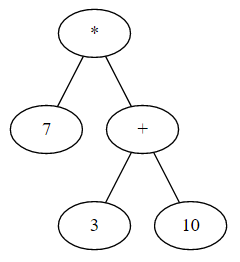
\includegraphics[width=0.4\linewidth]{figure/syntax_exempel_bild.png}
  \caption{Ett exempeluttryck från syntaxträdet illustrerat i ett
           träddiagram.}\label{fig:syntax_exempel_bild} 
\end{figure}

Precis som semantik har en roll i samband med syntax, har semantik även en roll
i samband med syntaxträd. I detta exempel är semantiken det värde som
syntaxträdet betyder. Detta värde kan beräknas utifrån syntaxträdet. Det görs
genom en \textit{beräkningsfunktion}. För exemplets syntaxträd kan
beräkningsfunktionen se ut som i figur \ref{fig:eval_tree}

\begin{figure}[tph]
  \begin{lstlisting}
evaluate :: Expr -> Double
evaluate (e1 :+: e2) = evaluate e1 + evaluate e2
evaluate (e1 :*: e2) = evaluate e1 * evaluate e2
evaluate (Const v)   = v
  \end{lstlisting}
  \caption{En beräkningsfunktion för syntaxträdet.}\label{fig:eval_tree}
\end{figure}

Det finns tre saker som är speciellt värda att notera i
figur~\ref{fig:eval_tree}. Den första är att eftersom syntaxen innehåller tre olika
typer av element, här motsvarat av de tre datakonstruktorerna, krävs tre fall i
beräkningsfunktionen som beräknar vardera av dem. \texttt{evaluate} har
därför ett fall för \texttt{:+:}, ett för \texttt{:*:} och ett för
\texttt{Const}. 

Den andra saken att notera ur figur~\ref{fig:eval_tree} är hur ett fall
beräknas. Hur beräkningen ska se ut får man genom att ta hänsyn till
semantiken hos det syntaktiska elementet. \texttt{e1 :+: e2} är syntax för
addition av de två uttrycken \texttt{e1} och \texttt{e2}. Därför blir
semantiken, värdet, av \texttt{e1 :+: e2} lika med värdet hos \texttt{e1} och
\texttt{e2} adderade. Ett liknande resonemang ger svaret på hur beräkningen av
de två resterande fallen ska se ut.

Den tredje saken i figur~\ref{fig:eval_tree} värd att poängtera är dess
typsignatur, \texttt{Expr -> Double}. Den gör nämligen att man kan tolka
\texttt{evaluate}, och beräkningsfunktioner i allmänhet, som en översättning
från syntax (här \texttt{Expr}) till semantik (här \texttt{Double}).

\end{draft}

\section{Litterat programmering och Literate Haskell}\label{sec:lhs}
\begin{draft}
\textit{Litterat programmering} (engelska \textit{literate programming}) är ett
alternativt sätt att programmera som introducerats av Donald Knuth~\cite{knuth}.
Istället för att skriva ett program för en dator, skriver man ett program som
kan läsas både av människor och datorer. Det visar sig bland annat på följande sätt.

Jämfört med traditionella program får dokumentationen en
ökad betydelse. I traditionella program är programkoden den viktiga delen. I
litterata program är däremot dokumentationen minst lika viktig. Den används till
att förklara koden, sätta den i relationen till andra delar, med mera.
Detta jämnbördiga förhållande syns konkret genom att titta på hur källkoden är
skriven i ett litterat program. Det kan till exempel se ut som i
figur~\ref{fig:litterate_haskell_exempel} där man ser att källkoden och
dokumentationen är sammanvävda på ett jämnbördigt sätt, där den ena inte är
viktigare än den andra.

\begin{figure}[tph]
  \begin{lstlisting}[language={}]
How does all this tie together? First the type is decided, for instance

> type ExampleType = Quantity T.Length Double

then a value of that type is created

> exampleValue :: ExampleType
> exampleValue = Quantity V.length 5.3

Note that the Quantity data type has both value-level and type-level dimensions. As previosuly mentioned, value-level in order to pretty print and type-level to only permit legal operations.
\end{lstlisting}
  \caption{Ett exempel på hur en källfil till litterat programmering kan se ut, tagen direkt från det resulterande läromaterialet.
           Exemplet är Literate Haskell. Rader som börjar med \texttt{>}
           markerar att det är programkod, medan rader utan markerar att det är
           dokumentation.}\label{fig:litterate_haskell_exempel} 
\end{figure}
% OBS! Raden med "note that the quantity..." måste vara en lång rad. Annars blir det fel i PDF:en

%Det andra sättet ett litterat program skiljer sig åt är ordningen programkoden
%står i. Traditionell programmering börjar oftast med att definiera små funktioner
%och metoder med snäva användningsområden och använder sedan dessa för att senare
%bygga ihop mer komplexa strukturer. Med litterat programmering börjar man hellre
%med komplexa strukturer först och skriver text som förklarar den generella
%strukturen utan att gå in på detaljerna, för att sedan presentera de små
%delarna var för sig med tillhörande förklarande text.

\textit{Literate Haskell} är litterat programmering för Haskell~\cite{litterate_haskell}.
Att programmera i Literate Haskell går till på samma sätt som vanlig Haskell,
med skillnaden att programkod och text vävs ihop i en och samma fil. Det kan
se ut som i figur~\ref{fig:litterate_haskell_exempel}. Filen, med tillägget
\texttt{.lhs}, går att använda direkt med Haskell-kompilatorn GHC. All text
ignoreras och programkoden behandlas som om den var en vanlig
Haskell-fil. \texttt{.lhs}-filen kan också kompileras till en läsbar typsatt rapport eller hemsida.
Det finns flera verktyg som gör det men det som används i detta
projekt är \textit{Pandoc}~\cite{pandoc}. Med Pandoc kan texten märkas
upp med både \textit{Markdown} (används i projektet) och \LaTeX. Det går
att exportera till bland annat HTML (som i läromaterialet) och PDF (som i den här rapporten).
\end{draft}

\section{Att skapa motiverande läromaterial}\label{sec:arcs}
\begin{draft}
Motivation är en persons vilja att göra något. I undervisningssammanhang vill
man att studenten ska lära sig materialet. Studenten behöver alltså vara
motiverad, att vilja, lära sig. Motivation kan ha flera källor. Till exempel att
studenten tycker materialet är intressant eller att det finns belöningar i form
av tillfredsställelsen att få att högt betyg. 

\textit{Motiverande design} innebär att systematiskt utforma undervisningen på
ett sådant sätt att studenten blir motiverad till att vilja lära sig. Det handlar om
att använda olika tekniker för att väcka och behålla motivation. Det finns ett
flertal olika modeller för detta men i detta projekt används enbart den så
kallade \textit{ARCS-modellen}~\cite{arcs_book}.

\textit{ARCS} är en förkortning av ``Attention, Relevance, Confidence and
Satisfaction'', på svenska ``uppmärksamhet, relevans, självförtroende och
tillfredsställelse''. Precis som namnet antyder innehåller modellen fyra delar
som vardera behandlar en aspekt av motivation. \textit{Attention} handlar om att
fånga uppmärksamhet och väcka nyfikenhet. \textit{Relevance} handlar om att
tillgodose studentens behov så att materialet upplevs som relevant för hen.
\textit{Confidence} handlar om att övertyga studenten att hen kommer kunna
lyckas lära sig materialet. \textit{Satisfaction} handlar om att ge studenten
tillfredsställelse efter att ha lärt sig något så att hen vill fortsätta lära
sig. Det finns strategier för hur man genomför de olika delarna i praktiken och
här följer en översikt för \textit{Attention}.\footnote{Eftersom projektet har
ett begränsat fokus på de pedagogiska aspekterna, se
avsnitt~\ref{sec:avgransningar}, har enbart \textit{Attention}  tagits hänsyn till. Av detta skäl är det enbart denna
del beskriven här.}

För att fånga studentens uppmärksamhet och intresse finns tre allmänna
strategier. Den första är varseblivning, att något plötsligt händer som man
blir medveten om. Det kan till exempel åstadkommas genom överraskande
information, en förändring i ljuset i en föreläsning eller att humor vävs in.
Den andra är att väcka nyfikenhet. Ett par sätt för det är att involvera mystik
i miljön och att ställa frågor. Det tredje sättet är variation. Då handlar det
om olika struktur och ordning på utlärningen, till exempel att inte alltid
utforma en lektion som föreläsning, demonstration och sedan övning, utan variera
det med andra inslag, exempelvis ett filmklipp.

Utifrån det sociokulturella perspektivet som Vygotskij utvecklade~\cite{LSB_kap5}
lär sig elever av varandra. Eleverna befinner sig vid sin närmsta 
utvecklingszon, där eleverna kan hjälpa varandra att förstå innebörden av
definitioner och uttryck genom att sätta ord på det de vill kommunicera. Denna
typen av kommunikation skulle kunna tänkas hjälpa elever sätta fingret på det de
inte förstår. Med denna bakgrunden skulle parprogrammering kunna vara
fördelaktigt. Dels för att eleverna kan lära sig av varandra, att de genom att
kommunicera sin förståelse internaliserar ämnet och bygger en djupare
förståelse. Parprogrammering lämpar sig antagligen även för att begränsa
flyktförsök, där elever medvetet eller mindre medvetet börjar göra något annat.

%Jean Piaget - Kognitivismen (lära sig A, B, A + B -> C, alternativt att eleven utmanas med något den trodde var sant, och tvingas omformulera en lösning som stödjer den presenterade situationen). s157

Då internetplattformars interaktion med eleven är begränsad i jämförelse med då
eleven är i skolan och har tillgång till lärare, så brukar internetbaserade
läroplattformar förlita sig på behavioristiska element (former av respons) i form av rätt eller fel
svar~\cite{LSB_und}. Vårt läromaterial har visserligen ingen interaktiv sida,
men typsystemet i Haskell skulle ändå tänkas kunna fungera som en fingervisare
när man gör rätt eller fel. Det går exempelvis inte att räkna med dimensioner
på ett olämpligt sätt, och funktionskomposition fungerar endast om båda funktionernas
typdefinitioner (typer på argument och returvärde) stämmer överens 

Evolutionärt sett har snabba belöningar varit fördelaktigt framför långsiktiga
som kräver långsiktigt engagemang (exempelvis öva inför en tenta) vilket beskrivs i
boken ``Dansa på deadline: Uppskjutandets psykologi''~\cite{DPD}. Detta är ännu en
orsak till varför det är bra med belöning exempelvis i formen av glädje då man
ser att koden kompilerar. Läromaterialet innefattar även strategiskt placerade
roliga bilder, för att ge impulsiva reaktioner av glädje. Sporadiska belöningar

\end{draft}
